% DOCX paragraph 626
\chapter{Black Holes: Champions Of Curvature}\label{ch:06}

% DOCX paragraph 627

% DOCX paragraph 630
We saw in the previous chapter how the advent of X-ray\index{X-ray!radiation} astronomy at
the end of the 1960s left astrophysicists ``bewildered''. The observations obtained by
X-ray\index{X-ray!radiation} satellites revealed the existence of never-before-seen objects,
with very large masses but extremely small in size. Sources such as Sco
X-1\index{Scorpius X-1 (Sco X-1)} and Cyg X-1\index{Cyg X-1} represented inexplicable surprises
within astrophysics and called into question all that was understood of modern physics
at that time. To make matters worse, a plausible explanation by way of a hypothetical
``neutron star'' could be postulated for Sco X-1\index{Scorpius X-1 (Sco X-1)}, but the
phenomenology of Cyg X-1 represented a far more puzzling enigma.

% DOCX paragraph 631
With a mass of about 15 solar masses, it certainly was not possible to invoke the
presence of a neutron star for the observations of Cyg X-1\index{Cyg X-1}.
Furthermore, the variability\index{variability} of the X-ray\index{X-ray!radiation} emission
from Cyg X-1 (usually around one second, but potentially dropping to just a few
milliseconds) suggested the presence of a much more compact object, with a size in the
order of only a few tens of kilometres. Today, we know that Cyg X-1 is a fairly ordinary
representative of a whole class of celestial objects exhibiting the same phenomenology:
the high-mass X-ray\index{X-ray!radiation} binaries (HMXBs). Again, these are binary systems
in which there is a transfer of mass from an ordinary star to another much, much more
compact object. As with Sco X-1\index{Scorpius X-1 (Sco X-1)}, the transfer of matter in the case of
Cyg X-1 also occurs via an accretion\index{accretion disc} disc through which matter falls
onto the compact object, heats up, and emits very intense radiation in the
X-ray\index{X-ray!radiation} band. The most relevant difference between Cyg X-1 and Sco
X-1\index{Scorpius X-1 (Sco X-1)} is that, in the case of Cyg X-1, the ordinary star was the object
with the largest mass, while the other more compact member of the binary is what today
we know to be\ldots{} a \emph{black hole!}

% DOCX paragraph 632
These celestial bodies have become an integral part of the collective imagination and
general knowledge. In fact, so much so that a shrewd (and amusing) answer to the simple
question, ``What is a black hole?'' came from my little daughter Anna, who was not even
old enough to go to school at the time. Yet, as children often do, she addressed the
question with the superiority typical of someone who thinks they know everything about
life: ``Well, it's obvious! It's simply a hole that can't be filled~...''. This answer
is certainly not wrong --- actually, it is perfectly true because normally a hole can be
filled. However, it remains a purely qualitative description, which unfortunately does
explain what black holes are. Since it is not uncommon that information found on black
holes is confusing or even misleading, it may be helpful to put some order to what you
may already know.

% DOCX paragraph 633
Thus, to remove some of the urban myths and most superficial descriptions of black
holes, I will endeavour to provide a clear and gradually detailed explanation of what
they are and the properties they possess. I will begin with their genesis and end with a
discussion of the difficulties that scientists still have in managing a concept that is
fundamentally difficult to accept.

% DOCX paragraph 638
\section{An Utterly Bizarre Solution}\label{sec:06-solution}

% DOCX paragraph 640
A simple yet rigorous approach to explain black holes could come from their definition
and, in particular, from the fascinating, albeit tragic, genesis of what turned out to
be the first solution to the Einstein equations, found by Karl
Schwarzschild\index{Schwarzschild!Karl} (1873-1916), a physicist from Frankfurt am Main.

% DOCX paragraph 641
I recall that in November 1915, in the proceedings of the then Royal Academy of Sciences
in Berlin, Albert Einstein published his field equations, the foundation of his theory
of general relativity\index{general relativity}. At that time, Karl Schwarzschild was already a
renowned astronomer; indeed, he was the director of the Astrophysical Observatory in
Potsdam, a few kilometres from Berlin. Despite holding this prestigious role, like many
German Jews of his generation, Schwarzschild felt the need to express his loyalty to
Germany and the sense of belonging that bound him to German society. Consequently, at
the outbreak of the First World War in 1914, he enlisted as a volunteer and was sent to
fight. Although already aged 40, he was sent to the western front, and then to the
eastern front. Unfortunately, due to the harsh conditions encountered in Russia, he
became seriously ill, and his health quickly deteriorated. He died in 1916 but, in the
last months of his life, he managed to find the first solution to the Einstein
equations.

% DOCX paragraph 642
Unaware of the impact it would have, Schwarzschild gave no name to his
solution\index{Schwarzschild!solution}. In 1967 (another significant event that year~...) the
American physicist John Archibald Wheeler used the descriptive term ``black
hole\index{Schwarzschild!black hole}''.\textsuperscript{\hyperlink{note:06-01}{1}} Although Schwarzschild's findings represent
the simplest solution of the field equations of general relativity, it is only possible
for me to cover this topic in the final part of my course on general relativity in
Frankfurt, after spending months on introducing all the mathematics necessary for its
derivation. Let me remind you of the three important hypotheses under which this
solution can be found:

% DOCX paragraph 644
\begin{enumerate}
\item the presence of a spherical symmetry\index{spherical symmetry};

% DOCX paragraph 645
\item the independence from time, i.e., the solution is static;

% DOCX paragraph 646
\item the absence of matter, i.e., the solution is in a vacuum\index{vacuum}.
\end{enumerate}

% DOCX paragraph 648
We now know that Schwarzschild's is also the \emph{only} solution to the Einstein
equations that satisfies these conditions (this is the thesis of the famous
\emph{theorem} by George Birkhoff\index{Birkhoff, George}, which we will discuss later).
However, it is unlikely that Schwarzschild himself fully appreciated the disruptive
novelty or the implications of his solution. Like many scientists after him, he must
have considered it an ``oddity'' of the new theory, to the point that he quickly entered
into intense correspondence with Einstein, asking for his opinion.

% DOCX paragraph 649
There are several aspects of Schwarzschild's solution that make it seem rather bizarre
to say the least. First, it is spherically symmetric, and therefore it has a ``centre''
and a ``far-away'' region (also referred to as the \emph{asymptotic}\index{spacetime!asymptotic}
region). In this region, and thus at large distances from the centre, the Schwarzschild
solution is not particularly strange, being the same as that of a source of gravity in
Newton's theory of gravity. However, while in Newton's theory, this result is possible
only in the presence of matter (since an object with mass has to produce the
gravitational field), the Schwarzschild solution is, as mentioned above, in a
vacuum\index{vacuum}. In essence, it suggests that it is possible to create a
gravitational field from \ldots{} nothing! A decidedly extravagant idea.

% DOCX paragraph 650
A second oddity is that it predicts the existence of a spherical surface with radius
\emph{r=r\textsubscript{S}} whose value is given by the following equation:

% DOCX paragraph 652
\begin{equation}\label{eq:06-01}
r_{S}=2M\textcolor{gray}{\frac{G}{c^{2}}}
\end{equation}

% DOCX paragraph 654
Exactly at this radius, also known as the \emph{Schwarzschild}\index{Schwarzschild!radius}
\emph{radius} and representing one of the fundamental length-scales in astronomy, a
number of strange phenomena occur, which we will discuss shortly. However, the most
peculiar and disturbing of these phenomena is that the Schwarzschild solution is not
well defined at this radius. From a mathematical point of view, the functions that
describe the solution at that radius \emph{diverge}, i.e., they assume infinitely large
values.

% DOCX paragraph 655
It is evident at first sight that Equation \eqref{eq:06-01} tells us the Schwarzschild radius is
equal to twice the mass \emph{M} of the object in question, i.e., the black hole (again,
I have greyed out the constants that do not have a ``physical meaning''). Today we know
that the Schwarzschild radius \emph{r\textsubscript{S}} represents the radius of the
so-called \emph{event horizon}\index{event horizon} (more on this later) and that the
divergence of the solution at this radius is not particularly worrying; it is simply the
result of an inadequate choice of coordinates\index{coordinates}. Indeed, it is possible
to use a whole set of better-suited coordinates that ``eliminate'' this
singularity\index{singularity!coordinate} and make the radius \emph{r=2GM/c\textsuperscript{2}}
perfectly regular, that is, without divergences.

% DOCX paragraph 656
However, other peculiarities remain at the Schwarzschild radius. In particular, it is
impossible for a ray of light emitted at this radius (but also for any object with mass)
to move outwards to larger radii, although the ray can move inwards. In other words, the
spherical surface with a radius equal to the Schwarzschild radius behaves as a
unidirectional membrane, allowing the absorption of objects, but not letting anything
escape. Later on, we will see what this means from a physical point of view.

% DOCX paragraph 657
Finally, a third oddity of the Schwarzschild solution --- one with the most serious
complications --- is that it also diverges at the centre, i.e., at \emph{r=0}. However,
unlike the singularity at the horizon, this one in the centre is much more severe and
cannot be ``healed'', even through an intelligent transformation of
coordinates\index{coordinates}. Instead, all the possible indicators of what happens when
one approaches the zero radius suggest that every physical and geometrical quantity
becomes infinitely large there. For this reason, \emph{r=0} has the fascinating but
somewhat disturbing name of \emph{spacetime singularity}.

% DOCX paragraph 658
Today we refer to the point \emph{r=0} in the Schwarzschild solution as a \emph{physical
singularity}\index{singularity!physical}, that is to say, a point of spacetime where the equations
of general relativity\index{general relativity} are impossible to solve because they are
divergent. In turn, this means that near the singularity, the laws of physics cease to
be valid, and we are therefore unable to predict or even understand what might happen
there. The physical singularity\index{singularity!physical} still remains the biggest thorn in the
side of Einstein's theory: the clear manifestation of the fact that, however correct the
theory may be, it remains incomplete. Indeed, although general relativity has been
proven to provide correct predictions on the behaviour of gravity on large scales, it
remains unable to describe gravity in the presence of very small dimensions and large
curvatures, i.e., scales at which the laws of quantum mechanics\index{quantum mechanics} come
into play. Even today, despite the efforts of generations of theoretical physicists, we
lack a theory of \emph{quantum gravity}\index{quantum gravity}. But, fear not, we will return
to this point at the end of our journey.

% DOCX paragraph 659
So, when proposed in 1916, the Schwarzschild solution triggered mixed reactions. On the
one hand, it showed that the Einstein equations were extremely interesting and had
solutions and, on the other hand, it raised more questions than answers. As you can
imagine, given its oddities, perhaps Schwarzschild's solution was a poor way to begin to
understand the consequences of general relativity\index{general relativity}. This may be why the
scientific community of those years received the new theory proposed by Einstein with an
attitude of detached interest and sceptical curiosity. This was true for the
mathematicians, who were attracted by the theory's geometrical implications, and the
physicists, who were instead interested in the experimental impacts.

% DOCX paragraph 660
The scientific climate of those years was characterised by a courteous appreciation of
the theory as well as a fundamental indifference to it, made worse by the difficulty in
finding solutions and thus understanding the predictions. Hence, the theory of general
relativity became the ``victim'' of a widespread lack of interest on the part of the
scientific community. However, such a feeling was not unreasonable and was in part
fuelled by some important ``distractions''. At that time, an equally compelling theory
had begun to attract the attention of the physics community --- \emph{quantum
mechanics}\index{quantum mechanics} --- another fascinating theory seeking to unveil the
properties of elementary particles. This new theory was also bizarre but had the major
advantage of offering much easier predictions to understand and, above all, to verify
through experiments.

% DOCX paragraph 661
As a result, during the first years of its existence, Einstein's theory seemed doomed to
slip slowly into oblivion. Fortunately, the advent of X-ray\index{X-ray!radiation} astronomy
and the observation of objects such as Cyg X-1\index{Cyg X-1} forced the scientific
community, fifty years later, to reconsider its predictions.

% DOCX paragraph 664
\section{Escape Velocity, Event Horizon And Singularities}\label{sec:06-escape}

% DOCX paragraph 666
Having covered the main oddities presented by the Schwarzschild solution, we will now
try and understand them. In particular, we will discuss the event horizon, the peculiar
properties of this mathematical surface and, finally, the physical
singularity\index{singularity!physical} at the centre of a black hole.

% DOCX paragraph 667
First, to illustrate the features of the event horizon\index{event horizon}, it is helpful
to start from a phenomenon that we can experience directly. Let us imagine taking a
tennis ball and hitting it upwards, being careful to give it a trajectory that is as
vertical as possible. We will observe that the ball will decelerate given a certain
initial speed. More precisely, its speed will progressively decrease during the ascent
until it becomes zero at a precise point of its vertical motion. At that point, the ball
will stop rising and fall back, accelerating as it returns towards you. We know that the
maximum height reached by the ball is directly linked to the force with which we have
hit it. Indeed, if we relaunch the ball with a different speed, the maximum height
reached when the motion is reversed will change. In particular, this height will be
lower if the initial speed is lower, and higher if the starting speed is higher.
Therefore, it is clear that there is a precise relationship between the initial speed
with which we hit the ball and the maximum height it reaches. In physics, we like to
think that the height represents the position where the ball's initial kinetic energy
(the energy it has because of its motion) is converted entirely into gravitational
potential energy, that is, the energy it has because of its position.

% DOCX paragraph 668
The most important aspect of this simple example is that there is a reason why the
tennis ball falls back, and this is because it is \emph{gravitationally bound}
\index{gravitationally!bound}. In other words, the gravitational field produced by the Earth is so
dominant over the dynamics of the ball that it is unable to escape from it. Following
this line of thought, we may ask ourselves if we could use an initial speed that would
allow the ball to escape\index{escape velocity} the gravitational field or become
\index{gravitationally!unbound}\emph{gravitationally unbound}. The answer is yes and is what we call,
unsurprisingly, the \emph{escape velocity}. Calculating its value is quite simple and
requires comparing the kinetic energy\index{energy!kinetic} with the gravitational potential
energy\index{energy!potential (gravitational)}. In this way, we obtain an expression that is valid in both
Newton's and Einstein's theory of gravity, namely:

% DOCX paragraph 670
\begin{equation}\label{eq:06-02}
v_{f}=\sqrt{2\frac{M}{R}\textcolor{gray}{G}}
\end{equation}

% DOCX paragraph 672
The expression above tells us that, given a source of a gravitational field with mass
\emph{M} and radius \emph{R} (for example, the Earth), the escape velocity is
proportional to the square root of the mass and inversely proportional to the square
root of the radius of the source. The escape velocity grows with the mass of the planet
(the more massive the latter, the greater the speed necessary to escape it), and it
decreases as the size of the planet increases.

% DOCX paragraph 673
Putting down some numbers, if we wanted to hit our tennis ball so that it escaped the
Earth's gravitational field, we would need to launch it with a speed of 11.2 kilometres
per second, or 40,320 kilometres per hour. A speed so high that not even the best tennis
player could ever send a ball into orbit on our planet, which is quite fortunate as it
would be very frustrating to watch a tennis match in which players cannot hit the ball
too high for fear of losing it!

% DOCX paragraph 674
That said, Equation \eqref{eq:06-02} is interesting for at least two reasons. The first is that the
escape velocity is independent of the mass of the ball we are hitting (only the mass of
the source of the gravitational field appears in the formula). In other words, to send
either a grain of sand or a spaceship to the Moon\index{Moon} requires the same
velocity (obviously, the energy spent to do so would be very different~...). The second
reason is that, as you may have noticed, the escape velocity depends on a quantity that
we have already encountered: the compactness \emph{M/R} of the source of the
gravitational field. This means that different celestial objects (the Earth, the Moon,
the Sun \ldots) will have different escape\index{escape velocity} velocities because their
compactness and, consequently, their gravitational fields are different. Indeed, the
escape velocity on the Moon is almost five times smaller than on Earth ---about 2.4
kilometres per second. Hence, even on our natural satellite, we would not be able to hit
the ball out of the gravitational field with the simple force of our muscles, but we
would undoubtedly hit it much higher than on Earth. Conversely, if we tried to do this
on the Sun, it would be difficult to hit it upwards at all, since the escape velocity
there is approximately 615 kilometers per second.

% DOCX paragraph 675
Incidentally, the very fact that the escape velocity on the Moon\index{Moon} is so
low --- lower than the average velocity of the molecules of nitrogen gas --- explains
why the Moon does not have an atmosphere. Luckily for us, the Earth's escape velocity is
large enough that it has retained an atmosphere, the presence of which is essential for
life on our planet.

% DOCX paragraph 678
\section{When The Escape Velocity Is As Large As Possible}\label{sec:06-light}

% DOCX paragraph 680
There is another aspect of Equation \eqref{eq:06-02} worth underlining. We know there is a maximum
speed at which objects can move: the speed of light. So, we can use formula \eqref{eq:06-02} to
calculate the compactness \emph{M/R} at which the escape speed velocity is equal to the
speed of light. If we do that, we will discover that, ignoring the constants \emph{G}
and \emph{c}\textsuperscript{2}, the value of the compactness\index{compactness!black hole} is
\emph{M/R}=\emph{1/2}. This result makes the Schwarzschild radius, as given by Equation
\eqref{eq:06-01}, much easier to understand: it is the radius of an object, more specifically a
black hole, whose compactness is \emph{M/R=1/2}, which is the maximum
compactness\index{compactness!maximum (absolute)} seen so far. This allows us to introduce a new definition
of the event horizon\index{event horizon} as the surface at which the
escape\index{escape velocity} velocity is the maximum possible, i.e., that of light. In other
words, if emitted exactly from the event horizon, light would not be able to leave the
gravitational field of the black hole because it would need an escape velocity greater
than the maximum allowed by physics.

% DOCX paragraph 681
Imagine now being on this mathematical surface and emitting a laser beam towards a
distant star. Due to the very strong gravitational field, the beam cannot propagate
outwards and instead will have to go back! I should emphasise that this behaviour would
only happen when sitting exactly on the event horizon. If we placed ourselves a little
further out and repeated the experiment, the gravitational field would still be
enormously strong, but part of our laser beam would be able to escape it and reach an
observer at a large distance.\textsuperscript{\hyperlink{note:06-02}{2}} Put another way, this peculiar behaviour
of light applies only as long we are at \emph{r=r\textsubscript{S}}; outside the event
horizon, i.e., at radii larger than \emph{r\textsubscript{S}}, the gravitational field
remains extremely intense, but it is not ``invincible''. Conversely, if we emitted a
beam of light within the event horizon, i.e., at radii smaller than
\emph{r\textsubscript{S}}, the beam would only move inwards, thus travelling towards the
centre of the black hole where the physical singularity\index{singularity!physical}is located.

% DOCX paragraph 682
Nevertheless, let us go back to considering the beam of light emitted just outside the
event horizon. We have seen that part of this beam would reach an observer even at a
considerable distance, for example, on Earth. However, the light perceived by such an
observer would be very different, in terms of colour (or wavelength), from that emitted
initially. Let's assume that, when emitted, the light was at a visible wavelength, say
in the \emph{blue} part of the spectrum\index{spectrum!electromagnetic}. The observer at a large
distance would instead receive it in the \emph{red} part of the visible spectrum!

% DOCX paragraph 683
Furthermore, this tendency of the light to ``appear red'' would be stronger the closer
the emission is to the event horizon. The wavelength of a light beam tells us about the
energy of the photons it is composed of; to be more precise, the
energy\index{energy!photon (of)} of a photon\index{photon!energy} is inversely proportional to its
wavelength. This process of the reddening of the light reveals that the light beam loses
energy when propagating from its emission point, near the event horizon, to the distant
observer.

% DOCX paragraph 684
This seemingly bizarre process actually makes perfect sense if we go back to thinking
about our tennis ball being hit upwards. Also, when moving upwards, the ball loses
kinetic energy, which transforms into gravitational potential energy. At a certain
point, the ball is forced to stop exhausting all its kinetic energy and has to fall
back. Since a photon\index{photon} cannot slow down because, by definition, it is
forced to move at the speed of light, it manifests this loss of energy by changing its
wavelength. I have just described a well-known phenomenon in astrophysics, which
reflects a very common property of the emission from compact celestial objects, namely,
the \emph{gravitational} \emph{red-shift}\index{red-shift (gravitational)}\index{gravitational!red-shift (see red-shift)}\emph{.}
This phenomenon is most extreme precisely in the case of black holes and becomes
mathematically infinite for a photon emitted from the event horizon. If the red-shift of
a photon emitted at \emph{r=r\textsubscript{S}} is infinite, the observer will never
receive it. Hence, the infinite red-shift experienced by a photon emitted at the event
horizon is a different way of understanding why a photon emitted at the event horizon
cannot propagate outwards but can, at most, remain on orbits\index{orbit} tangent
to this surface.

% DOCX paragraph 685
To make this concept as intuitive as possible, let's perform a gedanken experiment
together. Imagine yourself at some distance from the event horizon --- perhaps aboard a
spaceship positioned on one of the stable circular orbits\index{orbit!stable circular} (that are
allowed under the laws of general relativity) around a black hole --- and dropping a
device similar to a light on a buoy at sea, flashing at regular intervals towards the
celestial body. Well, as the buoy moves away from you and approaches the event horizon,
you will see that the interval between each flash increases, while the light produced by
the device, initially an intense white, will turn more and more to red. This process
will continue as long as a sufficient number of photons can reach you, but as time goes
by, you will receive fewer and fewer photons, and these will shift more and more to red.
At some point, when the buoy is very close to the event horizon, you will no longer see
any light, no matter how sensitive your instruments are. However, this does not mean
that the device stopped working or was destroyed before crossing the event horizon! If
you had been attached to the buoy, you would have seen that its flashes always had the
same periodicity, and the light did not change colour at all. Furthermore, after a
precise time interval that is simple enough to calculate, you would cross the event
horizon and find yourself inside it, unable to communicate with the universe outside.
Depending on the mass of the black hole, and especially if it were
supermassive\index{black hole!supermassive}, the passage through the event horizon would not even be
accompanied by any particularly dramatic event.\textsuperscript{\hyperlink{note:06-02}{2}}

% DOCX paragraph 686
This difference in the \emph{perception}\index{perception} of physical processes by
different observers (i.e., you observing the buoy from the spaceship; and you falling
together with the buoy) is a genuine property of general relativity --- from which its
name derives\index{general relativity}. Although this ``relativity'' of perception may seem
unsettling, it disappears when one does not discuss observational\index{observational!perception}
perceptions but the physical processes \emph{themselves}. When one does that, all
observers will agree on the same conclusion.

% DOCX paragraph 687
The example of the buoy teaches us that it is impossible to observe an event horizon (or
the birth of a black hole) \emph{directly} as long as such observations involve photons
and, thus, the emission and reception of light. However, it is still possible to obtain
\emph{indirect} evidence of the presence of a black hole, either through the emission of
electromagnetic radiation from its vicinity (as we will see in Chapter 7) or even
without any light and through the emission of gravitational waves (as we will learn in
Chapter 8).

% DOCX paragraph 688
At this point, I am aware that I have provided you with a lot of information about black
holes and their event horizons\index{event horizon}. So, let me briefly recap to put some
order and focus on the more essential points we have covered so far:

% DOCX paragraph 690
\begin{itemize}
\item It is possible to shine a beam of light outwards from a point very far outside the event
horizon: it will propagate, reaching regions placed at larger distances without
perceptibly changing its wavelength.

% DOCX paragraph 691
\item It is possible to shine a beam of light moving outwards from a point close to the event
horizon but still outside it, but part of it will bend backwards and fall onto the
horizon. As the emission of light takes place closer and closer to the event horizon,
the amount of light that fails to propagate outward becomes larger.

% DOCX paragraph 692
\item The light emitted near the event horizon will change wavelength, turning red due to the
gravitational red-shift effect\index{red-shift (gravitational)}. The strength of this red-shift
increases as its emission is made from points closer to the horizon and becomes infinite
for a photon emitted exactly at that surface.

% DOCX paragraph 693
\item A beam of light emitted from the event horizon, that is, a radius \emph{r=2M}, cannot
propagate outwards: if the black hole does not absorb it, its destiny is to remain
forever tangent to that spherical surface.

% DOCX paragraph 694
\item Unlike that of a neutron star, the event horizon is not a solid surface but a purely
\emph{mathematical} one. It is the boundary marking the transition between two physical
processes: one where a photon manages to propagate outwards and another where the
photon\index{photon} is instead forced to ``return''.

% DOCX paragraph 695
\item Much of what is said above for photons is also true for objects with a mass, which, on
approaching the event horizon, will need larger and larger energies to escape the
gravitational field. The energy required becomes infinite if the particle is placed
exactly on the event horizon.
\end{itemize}

% DOCX paragraph 696
I will conclude this discussion on a historical note. I have already mentioned that the
expression for the escape\index{escape velocity} velocity \eqref{eq:06-02} is also the same within
Newton's theory of gravity and was already known from the beginning of the eighteenth
century. Indeed, the British naturalist John Michell\index{Michell, John} (1724-1793) was
the first to formulate what could be considered an early idea of an event horizon. In an
article published in 1783,\textsuperscript{\hyperlink{note:06-03}{3}} he introduced the concept of ``dark
stars'': celestial bodies whose compactness was such that the escape velocity was equal
to that of light. With this remarkable foresight, such stars would not be able to emit
light! Of course, in 1783, general relativity was still to come, as was the concept of
the event horizon, and observations had not yet revealed the presence of objects such as
Cyg X-1\index{Cyg X-1}. Yet, it is quite incredible that ideas linked to black holes
were formulated (albeit in a somewhat embryonic form) centuries before these concepts
were put into sharp focus.

% DOCX paragraph 700
\section{When Time Makes Fun Of Us}\label{sec:06-time}

% DOCX paragraph 702
It is now time to face another physical phenomenon near the event horizon, which is
recurrent in all science-fiction films involving black holes: the
\emph{dilation}\index{dilation (of time)|see{time dilation}}\index{time dilation} \emph{of time}.

% DOCX paragraph 703
In Chapter 4, we saw how perfectly plausible it is that if mass or energy can bend
space, the same should also happen with time. Furthermore, we have said that the
wavelength of a photon emitted near an event horizon\index{event horizon} and directed
outwards is stretched out by gravity, causing what is known as gravitational
red-shift\index{red-shift (gravitational)}. So, now we just have to put these two concepts together.

% DOCX paragraph 704
To do this, I will use two hypothetical observers, Anna and Emilia, each onboard their
own spaceship orbiting a black hole on a stable circular orbit\index{orbit!stable circular} so that
neither of them runs any risk of falling into the black hole. Rather, they will maintain
a constant distance from the black hole, with Anna closer to the event horizon and
Emilia at a larger distance from it. Now, suppose that Anna emits a beam of blue light
directed towards Emilia: as we have seen, the latter will receive it without any problem
but at a reddish wavelength. We have interpreted this phenomenon as the consequence of
energy expended by the photon on exiting the gravitational well from which it was
emitted. However, there is another way to describe the same phenomenon. A photon is an
electromagnetic wave, and the number of crests associated with such a wave must be the
same for Anna, who sent it, and for Emilia, who received it. Furthermore, since the
photon must move at the speed of light, the change in wavelength can be interpreted as a
variation of the progress of time measured by Anna and Emilia. In short, the fact that
the two observers register different frequencies for the same photon\index{photon!frequency}
(remembering the frequency \emph{f} of a photon is inversely proportional to its
wavelength \emph{λ}: \emph{f} =\emph{c/λ} ) can be interpreted as the consequence of the
fact that the time taken to count the same number of crests is different for each
observer.

% DOCX paragraph 705
We have encountered something similar in Chapter 4 when discussing the slight difference
between clocks placed on the ground and clocks placed on satellites. Well, as with that
phenomenon, the gravitational red-shift\index{red-shift (gravitational)} experienced by Anna and Emilia
can be described as the manifestation of the elasticity of time. When comparing what
happens with the GPS, the important difference is that because Anna and Emilia are close
to a black hole where the curvature is extreme, they will register a much larger
(possibly extreme) variation in the progress of time. Indeed, this difference will
diverge near the event horizon. Put another way, the almost infinite red-shift suffered
by a photon emitted near the event horizon can be interpreted as being due to the
enormous ``slowdown'' of time as the photon\index{photon} tries to move outwards. To
clarify, the observer at a very large distance from the black hole will find time
progresses at the same rate it has in a flat spacetime. In contrast, for an observer
near the black hole, time progresses more slowly since that region of spacetime is far
more curved. Ultimately, time would virtually freeze for an observer on the event
horizon.

% DOCX paragraph 706
Perhaps we need to make use of another gedanken experiment to understand this concept
better. However, we will have to stretch the imagination a little further this time as
we find ourselves using extreme, albeit perfectly plausible, physical conditions.

% DOCX paragraph 707
So, let's imagine two astronauts, Carolin and Dominik, onboard a spaceship in a circular
orbit\index{orbit!stable circular} at a safe distance from a supermassive black hole, for example,
the one at the centre of the elliptical galaxy M87\index{M87!galaxy} (I will elaborate
on this fantastic object in Chapter 7). The two astronauts are bored and decide to take
a ``space trip'' on the smaller service spacecraft. Since much of the action in that
area occurs around the black hole (one way or another, it seems that everything
literally ends up falling into it!), they decide to get closer to it while remaining at
a safe distance from the event horizon. Both are well aware that there are safe orbits
for the small spacecraft, which can be calculated based on the power of their engines.
After checking everything is in order, they write a note in the electronic logbook, mark
the exact coordinates\index{coordinates}, including the astral date and time, and leave
the mothership.

% DOCX paragraph 708
The gravitational fields in the vicinity of a supermassive\index{black hole!supermassive} black hole,
such as M87*\index{M87*}, vary very gradually. To be more precise, the curvature
radius near these objects is extremely large, and differences between nearby locations
(i.e., the tidal fields) are quite small. So, instead of turning on the spacecraft's
rockets, Carolin and Dominik decide to simply enjoy their ``free
fall\index{free fall}'' as they are pulled towards the centre of M87. It is as if
Carolin and Dominik were gradually descending a mountain with enormous horizontal
dimensions and a very gentle slope. However, in reality, the gravitational attraction of
the black hole is so great that, even without their engines, Carolin and Dominik soon
reach very high speeds, close to that of light.

% DOCX paragraph 709
Meanwhile, sipping hot tea and tucking into fresh pastries, the two astronauts delight
in looking through the spacecraft windows at the breathtaking panorama of the matter as
it converges with them towards the black hole. Then finally, they decide it's time to go
back and the instruments confirm that, at their distance from the event horizon, they
can still reverse their course. So, they turn on the engines and point the spacecraft
towards the mothership, employing, it has to be said, a considerable amount of energy to
ascend the gravitational well into which they had gradually descended. In essence, the
climb away from the black hole is the difficult part~...

% DOCX paragraph 710
Once they reach the mothership, they check the instruments. The calendar marks a very
different astral date from that on which they left and that of their small spacecraft
--- according to the computer on the mothership, their trip lasted several months.
Carolin and Dominik, however, are not surprised; they knew this would happen, which is
why they took the fresh pastries with them rather than leaving them behind in the ship's
fridge. Of course, time passed much faster there than it did onboard the service
spacecraft, but it was a perfectly normal and totally predictable phenomenon for the two
astronauts. Actually, before leaving, Dominik had calculated the time they would
``measure'' onboard the small spacecraft to reach the event horizon or, had they decided
to cross it, the physical singularity\index{singularity!physical} at its centre. Aware of the
difference between ``their'' time on the small spacecraft and that measured by the
instruments onboard the mothership, he calculated the route, ensuring that the
difference between the two was not excessive: he did not want the mothership to remain
without a crew for too long. In short, this trip reveals that Carolin and Dominik are
familiar with general relativity and the subtleties of time in strong gravitational
fields.

% DOCX paragraph 711
That time can slow down and even stop seems absurd to us, so it can be helpful to
reflect on two important aspects of this phenomenon. First, we must never forget that
what seems implausible and even counterintuitive to us can be very plausible if allowed
by physics. Our intuition is built on experience accumulated on this planet, under
specific physical conditions, i.e., imperceptible curvatures, low temperatures and
densities, etc. Therefore, to establish what is physically possible, we must rely on the
equations that describe the laws of physics and do so almost blindly. If a theory is
correct and its equations allow a certain process to take place, then that process is
plausible (although not necessarily \emph{probable}).

% DOCX paragraph 712
The second aspect to keep in mind is that time dilation\index{time dilation} is not a
science-fictional invention but a reality on Earth supported by considerable
experimental evidence. In fact, we test its correctness every time we use a satellite
navigator. When compared to Carolin and Dominik's experience on their spacecraft, the
only difference is the magnitude of this phenomenon, which is enormously amplified in
the vicinity of a black hole or a neutron star. After all, it is precisely for this
reason that such objects fascinate us so much!

% DOCX paragraph 715
\section{How Do You Produce A Black Hole?}\label{sec:06-formation}

% DOCX paragraph 717
Now that we have a better idea of what a black hole is and what its most salient
features are, it is time to ask ourselves a basic but fundamental question: ``How are
these objects produced?''.

% DOCX paragraph 718
The answer is not exactly simple but not too complicated either, especially if you leave
out a few details, which is just what I intend to do in this section. Furthermore, I
will limit the discussion to black holes with a mass of between about three and 100
solar masses (typically called \emph{stellar}\index{black hole!stellar} \emph{black holes}) as
their formation process is much clearer than that of supermassive\index{black hole!supermassive}
black holes, whose cosmological origin is currently the subject of debate, and because
what I will say holds true in all cases, at least qualitatively. Also, I will take
advantage of what we learned in Chapter 5 about neutron stars and employ an invaluable
theorem to illustrate the process of black-hole formation.

% DOCX paragraph 719
But let's proceed in an orderly way. To explain how a stellar black hole is created, I
need to recall an important theorem by the German mathematician (also a naturalised
Australian citizen) Hans Buchdahl\index{Buchdahl, Hans} (1919-2010). The theorem is very
simple, and its thesis is expressed as follows: given a self-gravitating object made of
matter and having a mass \emph{M}\textsubscript{\(\star\)} and a radius
\emph{R}\textsubscript{\(\star\)}, its compactness\index{compactness!maximum (star)}
\emph{M}\textsubscript{\(\star\)}/\emph{R}\textsubscript{\(\star\)} is bound to be:

% DOCX paragraph 721
\begin{equation}\label{eq:06-03}
\textcolor{gray}{\frac{G}{c^{2}}}\frac{M_{\star}}{R_{\star}}\leq\frac{4}{9}
\end{equation}

% DOCX paragraph 723
In other words, given a self-gravitating object, its radius \emph{R}\textsubscript{\(\star\)}
must be greater than 9/4 = 2.25 times its mass \emph{M}\textsubscript{\(\star\)}. Note that the
theorem does not place a limit on the mass (which can therefore be tiny or huge) nor on
the radius needed to create a black hole. What it tells us, instead, is that for every
mass, whatever it is, there is a \emph{limiting radius} below which it is not possible
to find an equilibrium\index{equilibrium} solution to the Einstein equations.
Furthermore, the condition \eqref{eq:06-03} of the theorem also tells us that this limiting radius
is equal to 9/8 of the Schwarzschild radius, which, I recall, is \emph{r\textsubscript{S
}}=\emph{2GM/c}\textsuperscript{2}. Therefore, there is another way to describe the
implications of Buchdahl's theorem. It is impossible to arbitrarily reduce the radius of
a compact object with a solid surface and still obtain an equilibrium solution. Instead,
a limit is given by a radius that is only 13\% larger than that of the event
horizon\index{event horizon} of a black hole with the same mass.

% DOCX paragraph 724
The proof of the thesis of Buchdahl's theorem proceeds ``ad absurdum'', namely, by
showing that if an object made of ordinary matter, i.e., with a positive energy density
and pressure, were built with a compactness greater than 4/9, then the pressure at its
centre would be infinite. And since the pressure must necessarily be finite, it follows
that such an object cannot exist. Later on, we will see that, in principle, it is
possible to build objects with an even greater compactness. First, however, we need to
renounce an important assumption in the theorem and rely on a decidedly
\emph{exotic}\index{exotic!matter} type of matter.

% DOCX paragraph 725
This beautiful theorem offers us the opportunity for another of our gedanken
experiments. \index{neutron star!collapse to black hole} We can imagine taking an object with a mass
\emph{M}\textsubscript{\(\star\)} and progressively reducing its size in order to increase its
compactness. As I am sure you recall, we did something like this in Chapter 4, when we
imagined compressing the Sun to bring its radius to only five kilometres and then
calculated the resulting curvature. The experiment I am proposing here is similar, but
only in part because now we want to learn what happens when we exceed the limit imposed
by Buchdahl's theorem.

% DOCX paragraph 726
To help us in this gedanken experiment, we can use the three boxes in Figure \ref{fig:06-01}, which
show the curvature of spacetime produced by the Sun as we reduce its radius while
keeping the mass stable. Below each image, I have indicated the relative compactness
\emph{M/}R. The box on the left shows the curvature produced by the Sun with its true
radius of about 700,000 kilometres. As seen in Chapter 4, the
compactness\index{compactness} is of some parts in a million, and the curvature is almost
zero, so the surface appears flat. On the other hand, the middle panel shows the
curvature produced by compressing all the atoms of the Sun into an ultra-compact
star\index{ultra-compact star}, that is, to the limit set by Buchdahl's theorem. In this case,
the compactness is exactly \emph{M/R}=4/9≃0.444, and the curvature is clearly visible: a
depression with very steep walls has developed in the centre of the surface.

% DOCX paragraph 729
\begin{figure}[htbp]
\centering
\[\begin{array}{@{}w{c}{0.2933\linewidth}@{}w{c}{0.2933\linewidth}@{}w{c}{0.2933\linewidth}@{}}\text{Sun} & \text{ultra-compact star} & \text{black hole}\end{array}\]

% DOCX paragraph 731
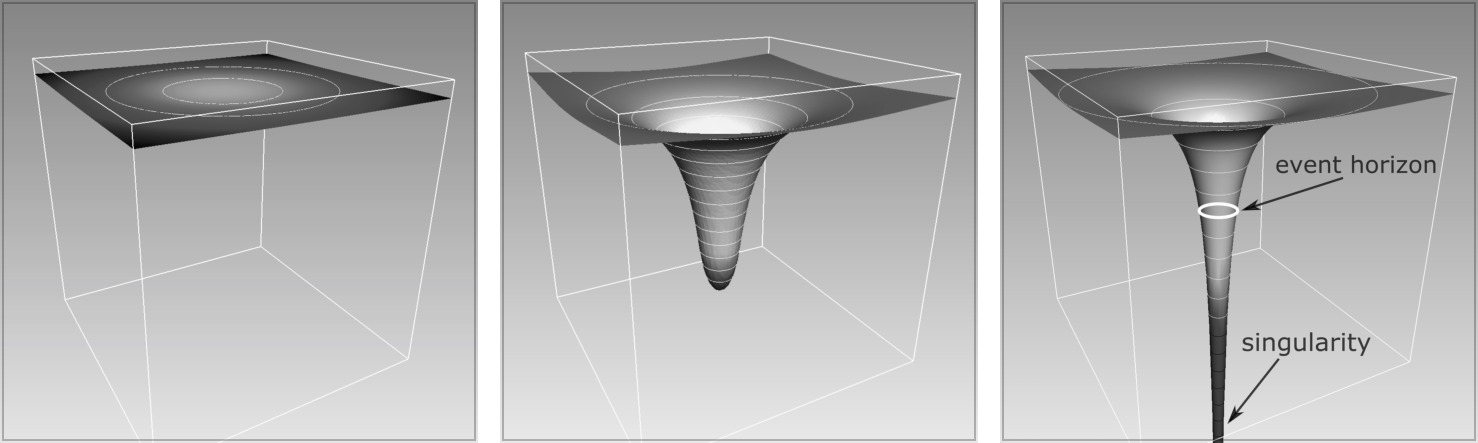
\includegraphics[width=0.88\linewidth,height=0.48\textheight,keepaspectratio]{../figs/pdf/en/fig-06-01.pdf}

% DOCX paragraph 733
\[\begin{array}{@{}w{c}{0.2933\linewidth}@{}w{c}{0.2933\linewidth}@{}w{c}{0.2933\linewidth}@{}}M/R\cong0.000002 & M/R\cong0.444 & M/R=0.5\end{array}\]

% DOCX paragraph 735
\caption{\emph{The curvature of spacetime produced by the Sun, on the left, is created
when we reduce its radius while maintaining its mass. The square in the centre depicts
the Buchdahl limit while, in the one on the right, its radius has been brought to just 3
kilometres, generating a black hole.}}\label{fig:06-01}
\end{figure}

% DOCX paragraph 737
Finally, the panel on the right shows what would happen if we took the ultra-compact
star\index{ultra-compact star} and compressed it further, even if only slightly, always keeping
the mass unchanged. This would produce an object with a spherical surface having a
radius of only 3 kilometres and a compactness of 0.5. That is, a black hole! When we
defined the Schwarzschild radius as being equal to twice the mass of the black hole in
Equation \eqref{eq:06-01}, we also implicitly stated that the compactness of a Schwarzschild black
hole\index{black hole!Schwarzchild} is exactly equal to \emph{M/R=1/2=0.5}. In the third panel of
Figure \ref{fig:06-01}, I have shown the position of the event horizon as given by a circumference
of radius \emph{r=r\textsubscript{S}} (a spherical surface appears here as a circle
because one spatial dimension has been suppressed). Also shown is the position of the
physical singularity\index{singularity!physical}, envisaged in the centre of the
``throat\index{throat}'', i.e., for \emph{r=0}, and therefore not visible in the
panel.

% DOCX paragraph 738
As you are now accustomed to doing, we can make a series of considerations inspired by
the sequence in Figure \ref{fig:06-01}. The first consideration is that we can use the panel on the
right (the black hole) to introduce a mechanical analogy to help you understand the role
gravity and the event horizon play. Imagine that the curved surface represents the bed
of a shallow lake, with a hole in its centre. The presence of the hole will create a
current that will drag the water of the lake towards the bottom, creating a huge
waterfall (let's ignore for the moment the presence of rotation, so the water does not
produce a vortex but falls along radial trajectories, just like a circular waterfall).
At this point, picture yourself on a boat with extremely powerful engines. As you get
closer to the waterfall, the current increases, but the engines on your boat are
powerful enough to push against the intense current, allowing you to approach not only
the outer edge of the hole but to go beyond the edge, even if the walls are almost
vertical. Well, this is possible only up to a certain point. In fact, there will be a
``border'' beyond which your engines will not be able to push you upstream, no matter
how powerful they are. Indeed, even if their power were almost infinite, it would not be
enough. Hence, for you and your boat, such a limit represents in all respects a
``horizon'': a surface you can cross but not leave!

% DOCX paragraph 739
The second consideration is that there are no intermediate solutions between the middle
and right panels in Figure \ref{fig:06-01}. In other words, if we compress, even infinitesimally, an
ultra-compact star\index{ultra-compact star} that has reached the Buchdahl limit, the Einstein
equations do not allow for any static solution other than that of the black hole.
Therefore, a sharp transition is created between the solutions of objects composed of
matter and having a solid surface, i.e., compact stars, and those without matter and
without a solid surface, i.e., black holes.

% DOCX paragraph 740
A third consideration, possible when looking at the curvature shown in the last panel,
is that it seems as if spacetime has been ``torn''; as if the very fabric of spacetime
has given way under the irresistible action of gravity. But, in reality, spacetime
cannot be torn apart since it is a regular continuum everywhere --- with the sole
exception of the physical singularity\index{singularity!physical} --- and we should instead think
that a black hole pushes its elasticity to the maximum. In other words, although we have
seen that spacetime is generally quite rigid, in the case of a black hole, gravity is so
strong that its deformability reaches its maximum value.

% DOCX paragraph 741
A fourth consideration emerges from the fact that in going from an ultra-compact
star\index{ultra-compact star} to a black hole, we have essentially concentrated all the matter
in a single infinitesimal point. Therefore, a black hole is ``empty'' since all the mass
used to generate it is now concentrated in a point of zero dimensions. It follows that,
with the exception of a point at the centre, the interior of the event
horizon\index{event horizon} is empty! Therefore, those statements suggesting the existence
of stable matter inside a black hole --- unfortunately discussed all too often --- are
incorrect. The density of matter in a black hole is precisely \emph{zero} because a
black hole is a solution of the Einstein equations in a vacuum\index{vacuum}.

% DOCX paragraph 742
To conclude, let me dedicate a final consideration to the timescale over which a black
hole is produced. I think it is now clear that nothing in physics happens
instantaneously, which also applies to the birth of a black hole. Equally clear is that,
within general relativity, this timescale inevitably depends on the position and motion
of the observer. Someone far from an event horizon will never see an object fall on it.
Likewise, someone far from a collapsing star will never see its surface disappear below
the horizon itself. Rather, the observer will see a star progressively contracting while
emitting light that gets dimmer and dimmer and shifts more and more towards the red
until, when the emitted radiation is too weak to be received, it disappears. Instead, if
the observer were to fall together with the collapsing matter, the precise duration of
the collapse \index{gravitational!collapse}would depend in part on a series of factors, such as the
type of matter or its rotation. However, omitting unnecessary complications from the
start of the collapse and, therefore, from when gravity dominates every other physical
interaction, the collapse essentially takes place over the free-fall\index{free fall!timescale}
timescale. Calculating this timescale is very easy, employing a simple formula that can
be used for any object, large or small. Basically, the formula says that the free-fall
timescale is inversely proportional to the square root of the density of the collapsing
object. The denser the collapsing object, the shorter the free-fall time. In the case of
the Sun, our favourite example, the free-fall time is about 27 minutes. To put it
another way, if we could magically ``turn off'' all thermonuclear reactions inside our
star and allow it to collapse by removing all of its internal pressure, then the solar
surface would reach the centre in a little less than half an hour. A surprisingly short
time if we consider that matter on the surface has to cover the 700,000 kilometres
separating it from the centre of the solar core.

% DOCX paragraph 743
So far, all of the considerations are meant to help us imagine what must have happened
about five million years ago when the supernova\index{supernova} explosion of a very
massive star (over 40 solar masses) gave birth to the black hole in Cyg
X-1\index{Cyg X-1}. Indeed, the most relevant difference between what happens with a
supernova that gives life to a neutron star and one that generates a black hole is that,
in the latter case, the iron core\index{iron!core} is much more massive and of the
order of about ten solar masses. Under such conditions, the density reached during the
collapse\index{gravitational!collapse} is such that no pressure (not even that of the degenerate
matter discussed in Chapter 5) can counteract the eventual collapse of the stellar core.
Thus, when a sufficiently large amount of mass is concentrated within a radius of the
order of the Schwarzschild radius, a black hole will inevitably have to be produced.

% DOCX paragraph 744
Nowadays, thanks to the numerical solution of the Einstein equations and those of
relativistic\index{relativistic!hydrodynamics} hydrodynamics, we know quite precisely what happens in
the process of the formation of a black hole. Around 2005, together with European and
American colleagues, I myself studied this process, producing the first numerical
simulations to describe it in three dimensions, albeit when starting from some idealised
initial conditions. Despite these simulations, many aspects of the astrophysical genesis
of black holes, both in the case of stellar and of supermassive black holes, remain
unclear. In the case of stellar\index{black hole!stellar} black holes, electromagnetic
observations tell us they exist with masses between five and ten solar masses. In
contrast, the detection of gravitational waves\index{gravitational waves} so far (which we will
discuss in Chapter 8) suggests that they exist with masses between ten and 80 solar
masses. The situation becomes even more uncertain when we consider supermassive black
holes, that is, black holes of millions or more solar masses. There is far greater
uncertainty about the mass and cosmological era in which these are first produced.
However, it seems clear that, even when considering these enormous black holes, their
birth must at some point in time involve the condensation of enormous quantities of
matter into a region with a size comparable to the Schwarzschild radius. For this
reason, the gedanken experiment conducted previously remains perfectly valid for all
types of black holes and is a helpful reference, regardless of the mass of the black
hole under consideration.

% DOCX paragraph 747
\section{Black Holes Have No Hair}\label{sec:06-hair}

% DOCX paragraph 749
So far, I have always used mass as the only property for distinguishing black holes of
different types and have discussed small (or stellar\index{black hole!stellar}) and large (or
supermassive\index{black hole!supermassive}) black holes. However, it is reasonable to wonder if such
a complex object, described by equations that are extremely difficult to handle and even
more so to solve, can really be described only in terms of its mass. In other words, it
is time to ask ourselves: ``How complex are black holes?''.

% DOCX paragraph 750
To provide an answer, I need to digress briefly. As small children, our
perception\index{perception} of reality (and consequently our understanding of the
world) teaches us that a wealth of details inevitably accompanies complexity. It seems
obvious that a natural phenomenon with a complex manifestation must be full of
``properties''. To be clearer, let me turn to a few examples. Let's start from a context
known to all, at least on a general level: music. I think it is evident to anyone that a
symphony of classical music performed by a large orchestra is much richer in content
and, therefore, in nuance than the simple sound produced by a tuning fork. Because I am
aware that speaking of ``properties'' or ``richness of content'' may appear qualitative
and subjective, we should stick to a more objective measure. Therefore, consider the
number of instruments involved in a symphony of medium duration and multiply it by the
number of musical notes played during the symphony. This will give us a far more
quantitative and objective measure of the complexity of the symphony. The same
calculation can then be made for a tuning fork that repeats its note at regular
intervals over the same period of time. Using these more objective terms, it is then
trivial to conclude that the symphony orchestra is hundreds of times more complex than a
tuning fork.

% DOCX paragraph 751
It is possible to find similar examples within a biological context. For instance, we
could consider three living organisms we are familiar with: a bacterium such as
\emph{Escherichia coli}, a \emph{Drosophila fly,} and an \emph{earthworm}. These
organisms are obviously characterised by an increasing complexity since more and more
information is needed to describe them in this order. To quantify this complexity in
numerical terms, we could consider their genetic makeup: 5,000 genes for the
\emph{Escherichia coli}, 13,000 for the \emph{Drosophila fly} and 19,000 for the
earthworm (the number of genes in a human is of the order of 30,000). Because each gene
can be described in terms of a specific combination of amino acids, it is clear that an
enormous amount of information is needed to describe even the simplest of living beings.

% DOCX paragraph 752
In essence, therefore, both our daily experience and our knowledge of the world suggest
that the more complex an object, organism or physical phenomenon is, the greater the
amount of information needed to describe it. This would all make perfect sense if not
for the fact that black holes are a striking exception to this very reasonable rule.

% DOCX paragraph 753
Based on these examples, we could conclude that describing a black hole (the most
extreme result of the most complex equations of theoretical physics) would require an
enormous amount of information and that mass is just one of the innumerable properties
of black holes. Well, quite surprisingly, that's not the case: in reality, black holes
are the simplest macroscopic physical objects ever! This conclusion is the simple
consequence that to describe any black hole we need only \emph{three numbers}, which
embody as many properties. Once again, the concept of a black hole surprises us --- it
is immensely easier to describe than even the most elementary bacterium.

% DOCX paragraph 754
So, what are the three, and only three, properties of a black hole? They are the
mass\index{black hole!mass}, which we have already discussed; the
\emph{spin}\index{black hole!spin}\emph{,} namely the amount of intrinsic rotation; and,
finally, the electric charge\index{black hole!charge}. Generally, these properties are
represented by \emph{M} for the mass, \emph{J} for the spin angular momentum, and
\emph{Q} for the electric charge\index{black hole!mass}. Thus, we can assign any black hole a
place in the `database' of the universe by simply allocating to it the three values of
\emph{M}, \emph{J}, and \emph{Q.} In a realistic astrophysical scenario, the electric
charge of a black hole is expected to be essentially zero, so in practice, we can even
forget about the charge. The reason for this is easy to understand. If a black hole with
a net electrical charge of a certain sign was ever generated, the ever-present free
charges, i.e., the set of electrons, protons and other charged particles that circulate
freely in interstellar space (some of which would necessarily have the opposite sign to
the black-hole's charge), would be electrically attracted by the black hole and
absorbed. In this way, the charge of the black hole would quickly diminish until it
became zero. At that point, the black hole would be electrically neutral (i.e.,
\emph{Q=0}), and therefore unable to attract any other charge. This explains why, in
practice, astrophysicists use only two values, \emph{M} and \emph{J}, to describe these
amazing celestial bodies.

% DOCX paragraph 755
The spin angular momentum must be within a well-defined range to simplify things. For
this purpose, it is helpful to consider \emph{dimensionless} quantities, i.e.,
quantities that are defined in such a way that they have no physical dimensions
(kilometres, kilograms, etc.) and are therefore pure numbers. In this case, we can
define the \emph{dimensionless spin} of the black hole, given by the ratio between the
spin angular momentum and the square of the mass, namely, \emph{a=J/M}
\textsuperscript{2}. Well, for a black hole in general relativity this number must be
between -1 and +1 (the difference in sign reflects the orientation of the rotation with
respect to a reference axis and, thus, whether the black hole is rotating clockwise or
anti-clockwise). The quantity \emph{a} is zero in the case of a Schwarzschild black
hole\index{black hole!Schwarzchild}, which is, therefore, a \emph{nonrotating} black
hole\index{black hole!nonrotating|see{Schwarzschild}} (from here on, I will refer to it as either a
\emph{Schwarzschild} or \emph{nonrotating} black hole). However, if the dimensionless
spin \emph{a} has a non-zero value, I will refer to a \emph{rotating} black
hole\index{black hole!rotating|see{Kerr}}, or \emph{Kerr} black hole\index{black hole!Kerr} (after the New
Zealand mathematician Roy Kerr, who first found the solution\textsuperscript{\hyperlink{note:06-04}{4}}. As black
holes typically accrete matter that has a certain amount of angular momentum, in an
astrophysical context, black holes are always expected to be of the Kerr type, even
though some may be only slowly rotating.

% DOCX paragraph 756
The peculiar conclusion that only three properties describe a black hole is contained in
the famous ``\emph{no-hair theorem''}. The playful name, given by the aforementioned
John Wheeler and the Italian astrophysicist Remo
Ruffini\textsuperscript{\hyperlink{note:06-05}{5}}\index{Ruffini, Remo}, is aimed at underlining that if a black
hole is seen as a sphere, then it is devoid of details: just like one's head can be
devoid of hair\index{black hole!hair}. The thesis of the theorem, which is very simple to
formulate, essentially states that in general relativity a black hole that is isolated
and in an asymptotically flat spacetime (i.e., becomes flat at great distances) can be
described by just these three values: \emph{M}, \emph{J} and \emph{Q.}
Interestingly\emph{,} should something intervene to modify one of these numbers, for
instance, due to matter with angular momentum falling onto the black hole and changing
the values of \emph{M} and \emph{J}, the variation of the parameters will be followed by
a state in which all transient perturbations are removed, and a ``new'' black hole
remains, although different from the previous one, still described by values \emph{M},
\emph{J} and \emph{Q} (we will return to this point in Chapter 8).

% DOCX paragraph 759
\section{Cosmic Engines And Hawking Radiation}\label{sec:06-hawking}

% DOCX paragraph 761
In many respects, black holes can be seen as ``\emph{cosmic} \emph{engines}'' capable of
absorbing matter from the outside and thus modifying their mass, angular momentum and
electric charge (see Figure \ref{fig:06-02}). Indeed, three laws of ``black-hole dynamics'' exist
that tell us how, through interaction with the external world, the properties \emph{M,
J}, and \emph{Q} can change over time. Leaving aside the charge \emph{Q}, whose
evolution we have already discussed, these laws (which derive from a classical context
of general relativity\index{general relativity} without allowing for quantum mechanical effects)
tell us that the mass of a black hole can only increase. In contrast, its angular
momentum can increase or decrease, possibly becoming zero. In essence, a rotating black
hole can slow down and thus become a nonrotating hole through the loss of its rotational
energy. When this process occurs, a part of the mass of the black hole may actually be
reduced, but the total mass cannot be reduced entirely. More precisely, the part of the
mass associated with rotation (the part that depends on \emph{J}) can indeed decrease;
for obvious reasons, this part of the mass is also called the \emph{reducible
mass}\index{black hole!reducible mass}\index{mass!reducible}. However, there is a part of the mass of the
black hole not tied to rotation (i.e., that does not depend on \emph{J}) that cannot
decrease, but only increase. Again, for obvious reasons, this part of the mass takes the
name of \emph{irreducible}\index{black hole!irreducible mass} \emph{mass}\index{mass!irreducible}.

% DOCX paragraph 762
The law according to which a black hole, in the classical formulation of the theory of
general relativity, cannot lose its irreducible mass was revolutionised in the 1970s by
the British physicist Stephen Hawking\index{Hawking!Stephen}. He proposed a new mechanism
related to the principles of quantum mechanics\index{quantum mechanics} that indeed violates
this law.

% DOCX paragraph 764
\begin{figure}[htbp]
\centering
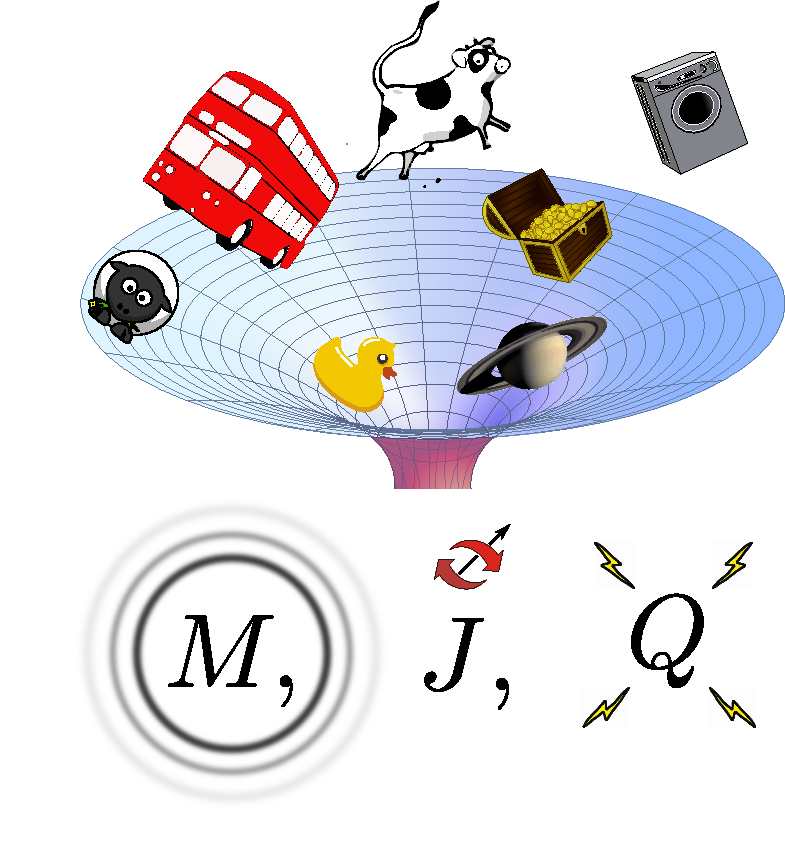
\includegraphics[width=0.88\linewidth,height=0.48\textheight,keepaspectratio]{../figs/pdf/en/fig-06-02.pdf}

% DOCX paragraph 765
\caption{No-hair theorem\emph{: regardless of the type of objects that black holes can
enhance, they only produce a change of the three numbers that characterise a black hole:
the mass M, the angular momentum J, and the electric charge Q.}
\index{black hole!mass}\index{black hole!spin}\index{black hole!charge}}\label{fig:06-02}
\end{figure}

% DOCX paragraph 767
Hawking suggested that a black hole could ``evaporate'' and, therefore, lose mass
(reducible and irreducible) through the emission of a thermal type of radiation, called
\emph{Hawking radiation}\textsuperscript{\hyperlink{note:06-06}{6}}\index{Hawking!radiation}\index{radiation!Hawking}. To
produce such radiation requires the generation of a series of virtual particles and
antiparticles (i.e., particles with ``negative mass/energy\index{energy!negative}'') in an
extremely thin region near the event horizon. We know that particles and antiparticles
can be produced anywhere in spacetime, with no net effect since the number of virtual
antiparticles produced is balanced precisely by that of the corresponding particles.
However, when the phenomenon occurs near an event horizon, which can only absorb
particles but not emit them, a net result is possible and the overall effect is that the
black hole emits radiation in terms of these virtual particles. At the same time, the
black-hole's mass decreases due to the accretion of antiparticles, which have negative
mass-energy and therefore contribute to a negative mass.

% DOCX paragraph 768
There is no experimental proof of the existence of Hawking radiation\index{radiation!Hawking}.
Of course, the main reason for this is that it is impossible to create a black hole in
the laboratory (although it is possible, in principle, to generate objects with similar
properties, called black-hole ``analogues''). But this is not the only reason: Hawking
radiation is, in fact, very weak, both in the case of stellar\index{black hole!stellar} black
holes and even more so for supermassive black holes\index{black hole!stellar}. More precisely,
\emph{Hawking's luminosity}\index{Hawking!luminosity}\index{ luminosity!Hawking}\emph{,} i.e., the amount
of mass-energy lost by a black hole per unit of time due to Hawking radiation, is
inversely proportional to the square of the black-hole's mass. It follows that even a
``light'' black hole, such as a black hole of one solar mass, would take about
10\textsuperscript{67} years to evaporate completely. Considering that the universe is
about 10\textsuperscript{10} years old, it is clear that a black hole of this mass would
take billions and billions and billions and billions of times the age of the universe to
evaporate. The timescales become even larger if we consider more massive black holes,
like that at the centre of our galaxy. That is why the best opportunity to observe
Hawking radiation comes from extremely small black holes. In particular, a black hole
that could have been generated in the early universe with a mass of
10\textsuperscript{11} kilograms (that is, one billionth of that of an asteroid) would
emit enough Hawking radiation to be on the verge of evaporating.

% DOCX paragraph 769
Despite this lack of observational evidence, the scientific community is unanimous in
believing that Hawking radiation\index{radiation!Hawking} is physically possible and that, at
least in principle, a black hole can also lose its mass, possibly disappearing
completely or leaving behind a very small singularity.

% DOCX paragraph 770
In summary, when talking about mass, black holes seem to behave just like humans: they
can sometimes ``lose weight'' if they slow down, but in the vast majority of cases, and
sooner or later, they inevitably tend to put on weight~...

% DOCX paragraph 773
\section{A Difficult-To-Digest Idea}\label{sec:06-idea}

% DOCX paragraph 775
The ``absence of hair'' in black holes presents a starting point for important
reflection on how the very notion of these objects, and particularly the existence of an
event horizon\index{event horizon}, is still hard to accept. An event horizon makes a black
hole decidedly ``\emph{exceptional}'', in the sense that it represents an
\emph{exception} to what we know and are accustomed to accepting in physics. Once the
mathematical surface of the event horizon is crossed, in fact, all information about the
properties of the object entering the black hole is simply lost; converted, together
with all of its complexity, into the only three properties an external observer can
measure: \emph{M}, \emph{J,} and \emph{Q}.

% DOCX paragraph 776
If you think about it, this behaviour is anomalous, to say the least, and certainly not
what we are used to in physics. Let me give you an example that illustrates how
exceptional this behaviour is. Imagine taking a few logs of wood and lighting a nice
bright fire; when the flames die down, all that remains of the wood are the fine
indistinguishable ashes. You might not think these ashes contain any information about
the original properties of the wood or the chemical properties of the organic cells that
constituted the wood. In essence, you would think it impossible to recover any traces
that would enable you to establish whether the wood logs came from a beech tree or an
oak tree. Any information would seem to have gone up in smoke!~... Well, that's
precisely the point! The ashes are not the only product of the fire, and it is possible,
at least in principle, to trace the properties of the wood by studying the gases
contained in the smoke produced during the combustion.

% DOCX paragraph 777
This example shows that while systems in physics can undergo transformations, the
complete information about the properties of the system is never lost. Of course, these
properties can (and do) change, and it is well possible that it can become increasingly
difficult to collect information on such properties (think of the smoke, for example).
However, for reasons at the very core of our understanding of physics, the information
on the system is never lost. The only exception to this basic logic is what happens
concerning a black hole! In this case alone, we lose all information about the
properties of what generated the mass, the angular momentum, and the charge of the black
hole, even though we had all this information right up until the event horizon was
crossed.

% DOCX paragraph 778
The inability to extract information from a black hole is called the
\emph{information-loss} paradox\index{information-loss paradox} and is much more serious than it might
appear. In fact, it undermines the very foundations of quantum
mechanics\index{quantum mechanics}, where the set of information in a physical system cannot be
lost. More precisely, this paradox arises because, when describing the state of a system
through a wave function (remembering a fundamental postulate of quantum mechanics is
exactly that the complete information of a physical system is contained in its wave
function), the evolution of this function must be unitary. In other words, having
specified the initial conditions of the system's wave function, its evolution is fully
determined. However, in the case of a black hole, this unitarity is violated so that
several initially distinct states would merge into one and become indistinguishable.

% DOCX paragraph 779
The information-loss paradox remains unsolved, despite decades of studies on the
subject. In fact, none of the theories introduced to remove it is convincing enough to
be accepted --- yet another strident confirmation of the incompatibility between
classical general relativity, as formulated by Einstein, and the principles of quantum
mechanics\index{quantum mechanics}.

% DOCX paragraph 782
\section{Giving Up A Cherished Method}\label{sec:06-method}

% DOCX paragraph 784
Another aspect makes the event horizon a rather ``indigestible'' concept for physicists.
If you remember, in Chapter 2, I stressed the importance of Galileo's work in defining
and introducing the scientific method\index{scientific method} --- the only beacon illuminating
human speculations. Over the centuries, Galileo's work has allowed us to reach firm
conclusions in the debates, some lasting for centuries, that inevitably characterise
scientific exploration: what is true and what is false, what is right and what is wrong.
Galileo himself summarised the importance of this method in one of his best-known
aphorisms. Turning to Tommaso Campanella, he declared: ``I prefer to find a truth,
albeit in a small thing rather than to argue about the greatest issues without obtaining
any truth''. In the case of a black hole, it is impossible to find a single truth, at
least in terms of the scientific method, about what is beyond the event horizon, and
this is not because the laws of physics cease to be valid!

% DOCX paragraph 785
Let me try and explain better what I mean. Imagine a pair of observers outside a
supermassive black hole; Simplicius\index{Simplicius} and
Salviati\index{Salviati}.\textsuperscript{\hyperlink{note:06-07}{7}} The two are arguing about whether or not
it is possible to conduct an experiment within the event horizon\index{event horizon}.
Following a logic of his own, Simplicius, who is not an expert in general relativity,
affirms that, after crossing the horizon of events, there lies a fantastic world where
no experiments are possible. Instead, everyone can get what they want there simply by
thinking about it. According to Simplicius, if he crossed that limit, he would find a
table laden with delicious foods and, in particular, his favourite ice cream (Simplicius
loves to eat, and everyone knows he cannot resist ice cream).

% DOCX paragraph 786
For Salviati\index{Salviati}, who knows general relativity well, none of this happens
inside the event horizon of a supermassive black hole. The laws of physics also remain
valid there, and any object that has entered has to end up in the physical
singularity\index{singularity!physical}, about which, he admits, he cannot make any prediction.
Salviati also argues that if the black-hole's mass is very large, then an object the
size of a human being will experience very small tidal forces\index{tidal forces} so that
no appreciable change will be experienced when crossing the event horizon. Except, of
course, for the fact that it will no longer be possible to communicate with the outside
world.

% DOCX paragraph 787
Now, based on our understanding of physics, we can all agree that
Simplicius\index{Simplicius}' thesis is far-fetched. It has no logical or scientific
support, and there is no reason to believe it to be correct. However, this is precisely
the problem; the discussion between the two cannot be resolved, even if it is ``a small
thing'' in Galileo's terms. The simple reason is that neither
Salviati\index{Salviati}, nor anyone else, can go inside the event horizon, verify
that there are no tables laid with delicious foods, and report the results to the rest
of the world. Even more irritating for Salviati is that he knows very well it would be
possible to \emph{carry out} an experiment disproving Simplicius' thesis, but the
problem would be communicating the results to the outside world since this is something
you are unable to do once inside the event horizon.

% DOCX paragraph 788
Accepting the existence of an event horizon is therefore equivalent to admitting the
presence, in our universe, of regions that are physically accessible but precluded from
an investigation based on a scientific method\index{scientific method}. This is not because
physics ceases to be valid there, since (at least in general relativity) the only
problematic region is a point of infinitesimal dimension at the centre of the black
hole. Therefore, much more trivial is the problem that the results of experiments
conducted within the event horizon cannot be disclosed --- a perspective that would
certainly make poor Galileo turn in his grave~...

% DOCX paragraph 789
If we want, we can resort to a somewhat risky analogy here. The event
horizon\index{event horizon} poses the same conceptual complications and philosophical
implications as the afterlife, something many believe in, but no one can prove because,
apart from well-known exceptions, no one has ever returned to tell us what there is
after death.

% DOCX paragraph 790
Such considerations demonstrate why the idea of an event horizon is so difficult to
digest for us physicists, who, through aspiration or ambition, wish to exercise
knowledge that extends to every corner of the universe. For us, the event horizon is
like a door that can be opened and passed through but then closes forever behind us.
This is why over the years, and in particular the last decade, a considerable
intellectual effort has been invested in the study of so-called black-hole
\emph{mimicker}\index{black hole!mimicker}\emph{s}. These are objects through which we try to
mitigate some of the conceptual difficulties posed by black holes, and which we will
have a closer look at in the next section.

% DOCX paragraph 793
\section{Observations vs Experiments}\label{sec:06-observations}

% DOCX paragraph 795
We have seen that the presence of an event horizon and a physical
singularity\index{singularity!physical} at its centre makes the very idea of a black hole
difficult to digest. Given these difficulties, you might ask: ``Is it possible to do
without black holes?''.

% DOCX paragraph 796
Many have grappled with this question, especially in recent years, with direct
observations of objects compatible with black holes made both through the detection of
gravitational waves (by the LIGO\index{LIGO}/Virgo collaboration) and thanks to
the first-ever ``photograph'' of a black hole (produced by the Event Horizon
Telescope\index{EHT (Event Horizon Telescope)} collaboration, or EHT).

% DOCX paragraph 797
Before addressing the answer, a more general consideration of how scientific knowledge
progresses is necessary, especially regarding astrophysics.

% DOCX paragraph 798
Astrophysics --- the only branch of physics providing evidence for the existence of
black holes --- is an \emph{observational} \index{science!observational}\index{observational!science} science
rather than an \emph{experimental} one\index{science!experimental}\index{experimental!science}. It is
impossible to carry out experiments in this branch of physics, unlike branches such as
solid-state physics or elementary particle physics. Put another way, in astrophysics it
is not possible to build an experimental device that allows one to produce, in a
controlled manner, the physical conditions under which a specific physical phenomenon is
expected to occur. By ``controlled manner'', I am referring to the possibility of
performing an experiment while having a clear idea of the errors that can affect the
measurements. Conversely, astrophysics necessarily relies on astronomical observations
to formulate theories, which can then be confirmed or refuted through additional
observations. This aspect of astrophysics (which is sometimes overlooked, if not
ignored) adds considerable complexity to the application of the scientific method for at
least two reasons.

% DOCX paragraph 799
The first is that it is generally difficult to predict the number of sources and their
properties that will be studied since only observations are made. By way of comparison,
when you build a particle accelerator like that at CERN\index{CERN}, once initial
conditions have been specified (e.g., the energy of the incident beam or the properties
of the target beam), you have an exact idea of the number of events or collisions that
it is possible to produce in a certain period of time. Unfortunately, in astrophysics,
it isn't that simple; unless you intend to repeat observations of well-known sources,
the construction of a telescope is usually accompanied by a great deal of uncertainty
about the number of new objects that will be observed. So, for example, when the
gravitational wave detectors of the LIGO \index{LIGO} collaboration went into
operation (not forgetting that gravitational wave astronomy is also an observational
science), the uncertainty about the number of events that could be measured was of three
orders of magnitude. In other words, it was not known whether there would be 400 events
per year or just 0.4.

% DOCX paragraph 800
The second reason scientific progress in astrophysics is more difficult is that, by
being an observational science, it suffers from a \emph{degeneracy}\index{degeneracy!intepretation} on
the possible explanations of the observations. Again, I will use an analogy to
illustrate this concept. Imagine an old wall clock in front of you, which you can
observe as much as you like. What would you notice about it? Probably that it has two
hands, one long and one short, and that the shorter hand rotates 360 degrees every 12
hours, while the longer one does the same every 60 minutes. Well, these are your
``observations''. Now, suppose you have to construct a mathematically complete and
physically plausible model of the internal mechanism that allows the clock to function.
As you can imagine, you could find many mathematical models and combinations of
mechanisms that can explain perfectly the rotation of the long hand every 60 minutes and
the short hand every 12 hours. However, only one of the possible explanations is the
right one, and it is even possible that you haven't considered it. Thus, to remedy this
apparent difficulty, you should use all your imagination and wit in an attempt to obtain
additional information. For instance, you could use microphones to listen to the
noise\index{signal|see{noise}}\index{noise} produced by the mechanism responsible for the
movement and use recordings to rule out models that are incompatible with ``acoustic
observations.'' Or you could measure the vibrations transmitted by the clock to the wall
and work on models compatible with this additional information.

% DOCX paragraph 801
Well, progress in astrophysics is achieved in a similar way. Also, in this field, all
available information is collected solely through observations, which scientists then
try to explain through mathematical models built based on the laws of physics.
Additional information can come from observations in different electromagnetic bands or
on different observational channels, in which case we refer to
\emph{multi-wavelength}\index{astronomy!multi-wavelength}\index{multi-wavelength astronomy} or
\emph{multi-messenger}\index{astronomy!multi-messenger (gravitational-wave)}\index{astronomy!multi-messenger}\index{multi-messenger astronomy}
\emph{astronomy}, respectively. And, as with the wall clock, those models that appear to
be more accurate and whose observations have more plausible explanations can turn out to
be incorrect precisely because there is a degeneracy\index{degeneracy!intepretation} between the
observations and the models capable of explaining them. Finally, the creativity of
astrophysicists enables them to use all the possible observations (and related
connections) to reduce the set of models that are in agreement with the observations or
to make predictions about the behaviours that, whether observed or not, could confirm or
refute the correctness of the model.

% DOCX paragraph 804
\section{Black-Hole Mimickers}\label{sec:06-mimickers}

% DOCX paragraph 806
Let's get back to the idea of black-hole mimickers. Our digression into the
epistemological aspects of astrophysics has been a useful illustration of how, even
though the black-hole solution represents the most natural and simplest explanation to
the phenomenology observed in compact astrophysical objects such as Cyg-X1, it is not
the only one. There are other explanations that do not require the presence of a black
hole. The characteristics of these alternative solutions are quite simple to guess. They
represent extremely compact objects without an event horizon or physical
singularity\index{singularity!physical}\textsuperscript{\hyperlink{note:06-08}{8}}. In fact, general
relativity\index{general relativity} and several ``\emph{alternative}\index{alternative theories (gravity)}
\emph{theories''} of gravity allow for a whole class of compact astrophysical objects
with these properties to exist; therefore, they are dubbed black-hole
\emph{``mimickers}\index{black hole!mimicker}\emph{''}. Indeed, their properties so closely
resemble those of black holes that sometimes they are almost indistinguishable from
them, at least in terms of measurements made by distant observers such as us.

% DOCX paragraph 807
Let's look in detail at some of these mimickers. Firstly, the so-called
\emph{gravitational star}\index{gravitational!star (see gravastar)}, or simply
\emph{gravastar}\index{exotic!compact object (gravastar)}\index{gravastar}. This is a solution of Einstein
equations in spherical symmetry\index{spherical symmetry} (perfectly compatible, therefore, with
what we know about general relativity) proposed in 2000 by physicists Pawel
Mazur\index{Mazur, Pawel} and Emil Mottola\textsuperscript{\hyperlink{note:06-09}{9}} \index{Mottola, Emil}. The
solution supposes the existence of a layered star with an inner core (essentially the
majority of the star) characterised by matter with quite unusual properties; unlike
everything we are used to, it has negative pressure\index{pressure!negative} (all the matter we
know of has positive pressure\index{pressure!positive}). Moreover, this core is surrounded by a
very thin ``skin'' of matter with equally extreme properties: an extra-strong but
positive pressure.

% DOCX paragraph 808
Negative-pressure matter can be considered as a small universe that wants to expand and
is associated with a ``de Sitter\index{de Sitter!spacetime} spacetime'', after the Dutch
scientist Willem de Sitter\index{de Sitter!Willem}, who first proposed it. Indeed, we believe
this solution of the Einstein equations is connected to the accelerated expansion we are
now measuring in cosmology. At the same time, however, the thin strip of matter at very
high pressure at the surface of a gravastar wants to collapse, counteracting the
expansion of the nucleus and generating a stable equilibrium. In other words, a
gravastar\index{gravastar} is like a balloon that has negative internal pressure but a
positive outward gradient! And in which the thin outer surface prevents the core from
expanding.

% DOCX paragraph 809
The most important peculiarity of this solution is that it can be constructed in such a
way as to have a compactness\index{compactness!gravastar} very close to the limit of a black hole,
only slightly below it, i.e., \emph{M/R} \(\lesssim \ 1/2\). In particular, it is
possible to build (as mathematical solutions at least) gravastars whose surface is just
above where the event horizon\index{event horizon} of a black hole with the same mass would
be, i.e., with a radius that is only infinitesimally larger than that of a Schwarzschild
black hole\index{black hole!Schwarzchild}. As a result, gravastars\index{gravastar} have a rigid
surface just like neutron stars (hence the name, gravitational ``star''), but do not
have any event horizon or contain any physical singularity\index{singularity!physical} at
\emph{r=0}; thus they are perfectly regular solutions.

% DOCX paragraph 810
The second example of a black-hole mimicker has become almost ``classic'': a
\emph{wormhole}. As with \emph{black hole}, its evocative name was also coined by John
Wheeler (in an article written with Charles Misner in 1957\textsuperscript{\hyperlink{note:06-10}{10}}).

% DOCX paragraph 811
Once again, this is a perfectly plausible solution of the Einstein equations for an
object in a vacuum\index{vacuum} and extremely compact, but whose
compactness\index{compactness!wormhole} is slightly less than that of a black hole. Interestingly,
because of the large curvature produced by wormholes, it is in principle possible to
join two regions of spacetime that are extremely distant and asymptotically flat. In
essence, the wormhole solution can be seen as a tunnel in the elastic fabric of
spacetime, providing us with a ``shortcut'' to connect two physically distant regions.
Imagine taking a section of a flat spacetime in two dimensions (our beloved sheet in
Chapter 3) and considering two points placed at a great distance from each other. If you
fold one end of the sheet to obtain two parallel layers, the two points would no longer
be so far from each other, which would be sufficient to be able to travel \emph{through}
the sheet instead of along it. Now, imagine a source of gravity intense enough to
distort the sheet, creating a double throat\index{throat}, and that's it: you have
created a shortcut between the two points that were far away from each other and are now
very close. It has long been shown that wormholes, at least in the simplest models, are
dynamically unstable; if opened, they would tend to close extremely quickly. At the same
time, there are wormhole solutions that can be stabilised by the presence in the throat
of exotic\index{exotic!matter} matter, i.e., with negative mass or
energy\index{energy!negative}.

% DOCX paragraph 813
\begin{figure}[htbp]
\centering
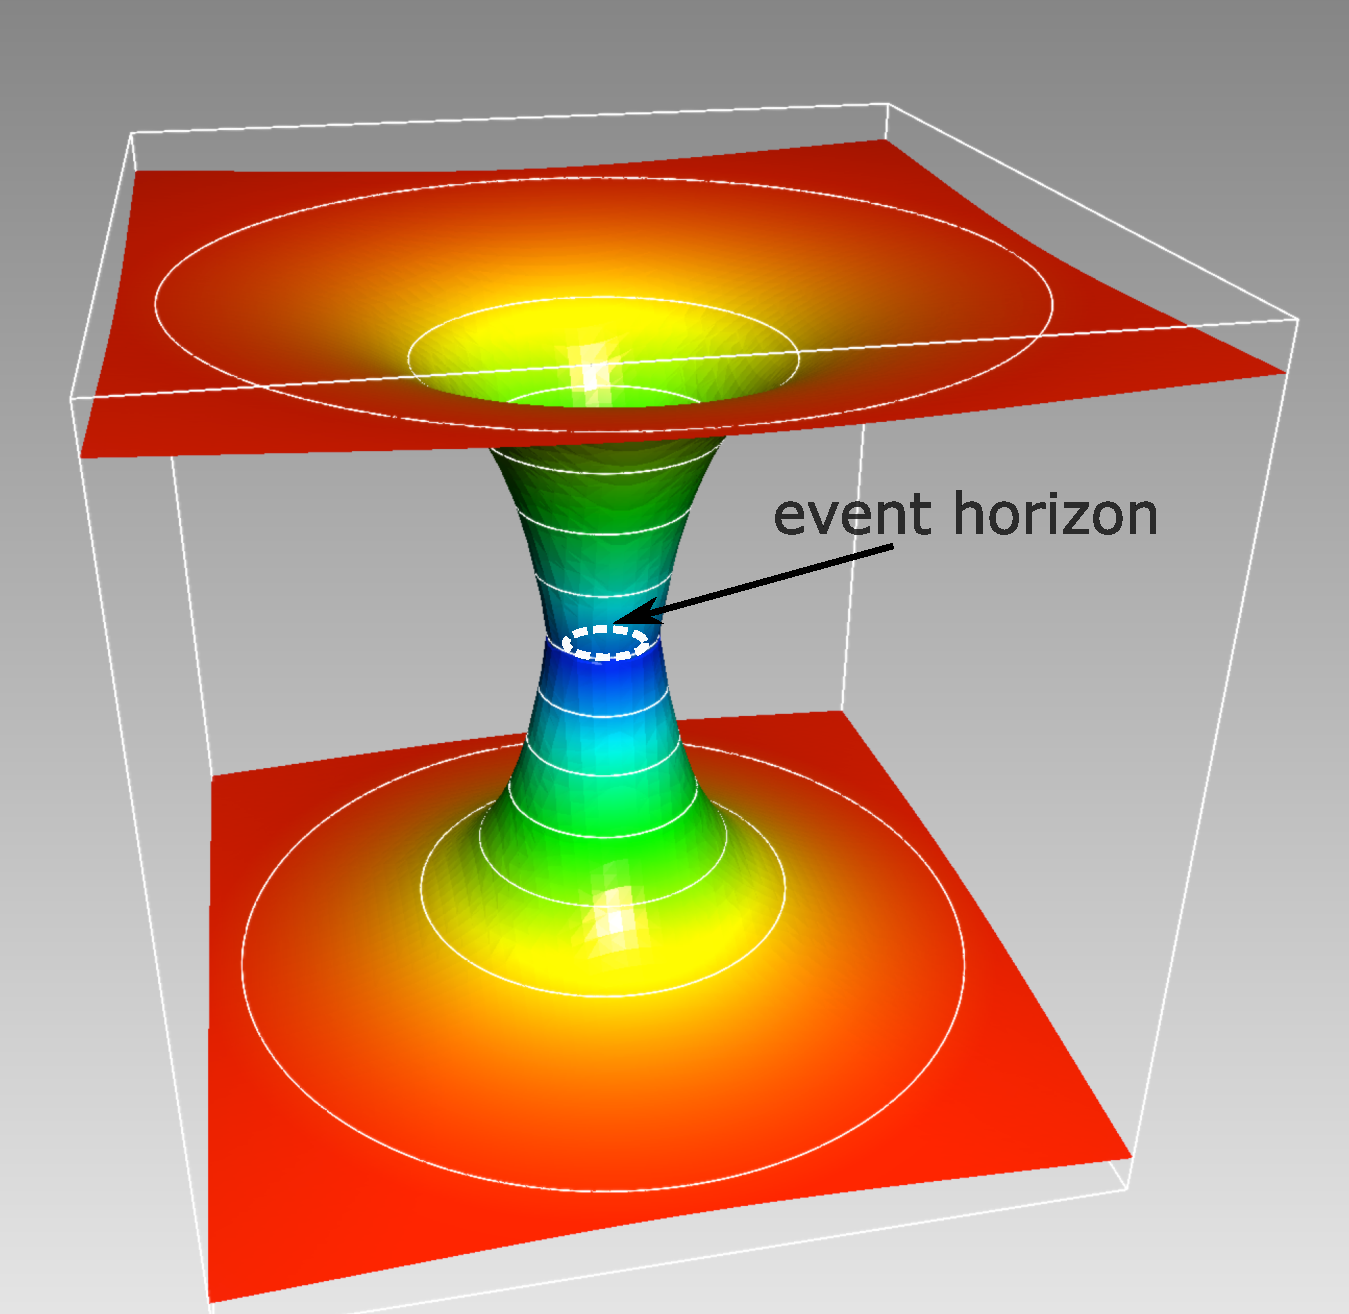
\includegraphics[width=0.88\linewidth,height=0.48\textheight,keepaspectratio]{../figs/pdf/en/fig-06-03.pdf}

% DOCX paragraph 815
\caption{\emph{Wormholes with two identical and symmetrical ``throats'' can join two
regions of spacetime that are flat at great distances. The smaller section of the
throat}\index{throat} \emph{is slightly larger than that of a Schwarzschild black
hole}\index{black hole!Schwarzchild} \emph{with the same mass.}}\label{fig:06-03}
\end{figure}

% DOCX paragraph 817
The schematic diagram of a wormhole reported in Figure \ref{fig:06-03} shows the typical
``throat\index{throat}'' we are used to in the presence of strong curvature. In this
case, however, the two throats are exactly symmetrical and can thus join two regions of
spacetime that are flat at great distances\index{spacetime!flat}. Nevertheless, it is
important to note that even in this case, the smallest section of the throat is slightly
larger than a Schwarzschild black hole\index{black hole!Schwarzchild} with the same mass would be (as
shown by the dashed white circle). Therefore, this is not a black hole but simply a very
compact object.

% DOCX paragraph 818
A gravastar and a wormhole differ significantly in at least one respect: the former has
a solid surface, like a neutron star, while the latter has no solid surface and, at
least in the simplest models, is actually a solution in vacuum\index{vacuum}. At the
same time, there are at least two properties that a gravastar and a wormhole have in
common. Firstly, both have an extremely high compactness, \emph{M/R,} very close to that
of a black hole, \emph{1/2}, but also slightly less. The second property they have in
common is their ``genesis''. In both cases, we only have a vague idea about how these
objects could be produced in nature. In other words, although gravastars and wormholes
are permissible and perfectly legitimate solutions of the Einstein equations, the
astrophysical processes that could lead to the formation of these objects are not known,
at least at present. The situation is very different for equally compact objects, such
as neutron stars or black holes. We have identified precise evolutionary tracks allowing
us to start from stars between 10 and 100 solar masses and to arrive, through a detailed
evolution of nuclear astrophysics, at a supernova\index{supernova} and, therefore, to
the formation of a neutron star or a black hole depending on the mass of the parent
star. However, even using the knowledge we have today of nuclear astrophysics and the
microphysical processes that can occur in a stellar context, it is not clear how it
would be possible to produce a gravastar or a wormhole in practice.

% DOCX paragraph 819
In an astrophysical scenario capable of generating these types of solutions, perhaps the
most serious complication is that both require the presence of exotic\index{exotic!matter}
matter. The properties of this matter (negative energy\index{energy!negative} or pressure)
manifestly contrast with those that characterise the matter we can experiment with on
Earth and access in the universe through astronomical observations.

% DOCX paragraph 820
Also, in this case, if we were to employ the severe logic of Occam's razor, we would
have to regard such solutions as unrealistic. However, suppose we put aside the
difficulties associated with the genesis of these objects for a moment. Then, it remains
clear that such solutions would have many of the properties we think characterise a
black hole. For this reason, if we return to the example of Carolin and Dominik's
journey towards the event horizon of a supermassive black hole, it would be very
difficult for the two astronauts to understand whether the object they are approaching
is a black hole or a gravastar. This is because the latter would behave in a very
similar way, generating an extremely strong gravitational red-shift and absorbing all
forms of light, at least in appearance.

% DOCX paragraph 821
Fortunately for us (although it couldn't be any other way for a physically acceptable
theory), general relativity enjoys the property of \emph{uniqueness}\index{uniqueness (solution)}
in its solutions. In other words, there cannot be two solutions of the Einstein
equations that are different but have identical properties. Although very similar, they
must necessarily differ in something and, therefore, possess at least one characteristic
that makes them distinguishable. For this reason (and thus to eliminate what would
otherwise be a disconcerting degeneracy\index{degeneracy!intepretation}), over the last few years,
scientists have studied in detail not only black-hole mimickers but principally the
aspects of these objects that make them distinguishable from actual black holes.

% DOCX paragraph 822
I, too, have been involved in research of this type and have shown, for example, that a
gravastar\index{gravastar} can be essentially indistinguishable from a black hole as
long as we test it using electromagnetic radiation. However, it is easy to tell a
gravastar from a black hole if we employ gravitational waves\index{gravitational waves}. Although
a gravastar and a black hole are similar in size, they have a radically different
interior; a gravastar is filled with exotic\index{exotic!matter} matter, while a black hole
is empty. Thus, once perturbed, the two objects will produce gravitational waves with
very different properties (we return to this subject in Chapter 7, when we consider
another exotic\index{exotic!compact object} compact object).

% DOCX paragraph 823
It is now helpful to return to the example of the clock hanging on the wall. We had
seen, in that case, how different models of internal mechanisms could be excluded
because they were inconsistent with the observations. Similarly, the task of modern
astrophysics is to produce models that use all the available information to explain the
observations and rule out alternative explanations that do not correspond with these
observations. Furthermore, approaches have been developed in recent years that are
``agnostic''. Therefore, they do not necessarily assume that the observed phenomenology
is a black hole, leaving room for alternatives such gravastars, wormholes, or any other
black-hole mimicker.

% DOCX paragraph 824
To conclude this chapter, it is important to remark on a very important concept. It is
true that a degeneracy\index{degeneracy!intepretation} exists in the explanation of the astronomical
phenomenology of objects like Cyg-X1. The alternative solutions have the very important
advantage of not suffering from any of the problems inherent with black holes (such as
event horizons or physical singularities). However, all things considered, the
black-hole solution remains the simplest and most natural explanation within the theory
of general relativity\index{general relativity}, which so far has always proved to be correct.

% DOCX paragraph 825
In addition (and this is a huge advantage over any alternative scenario), the genesis of
a black hole represents the natural conclusion of the sequence of events that we know
characterise the life of massive stars. It does not require improbable assumptions or
the presence of matter with properties that are radically different from those we are
used to. In other words, while the black-hole solution is admittedly hard to digest,
alternative solutions are in many ways even harder to accept.
